% Chapter 5

\chapter{ALGORITHMS} % Write in your own chapter title

After representing code solutions as feature vectors, the dataset was exported to perform training for machine learning models. The following models 

\begin{itemize}
    \item Support Vector Machine (SVM)
    \item Random Forest 
    \item Multi Layer Perceptron (MLP)
\end{itemize}

were employed for training. The detailed description of the mentioned algorithms are listed below. 

\section{SUPPORT VECTOR MACHINE}

In machine learning, Support Vector Machines are supervised learning models with associated learning algorithms that analyze data used for classification and regression analysis. Support Vector Regression \cite{D} is a supervised learning algorithm that is used to predict discrete values. Support Vector Regression uses the same principle as the Support Vector Machine (SVM). The objective of a support vector machine algorithm is to find a hyperplane in an n-dimensional space that distinctly classifies the data points. The data points on either side of the hyperplane that are closest to the hyperplane are called Support Vectors. These influence the position and orientation of the hyperplane and thus help build the SVM.

\subsection{Hyperparameters in SVR}

Following are the various key hyper parameters used in Support Vector Regression.

\begin{figure}[h]
\centering
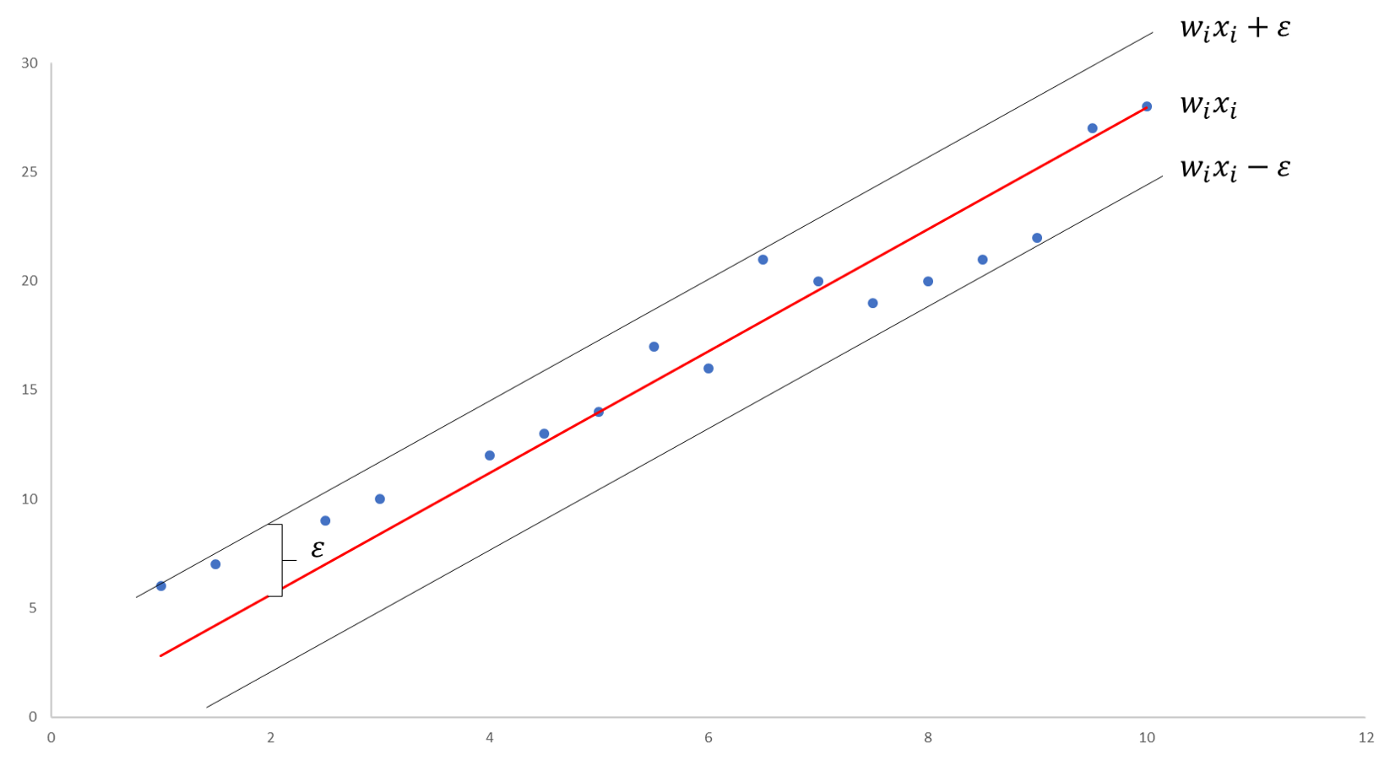
\includegraphics[width=1\textwidth, height=15cm]{./figures/svm.png}
\caption{Simple SVR}
\label{fig1}
\end{figure}

\begin{itemize}
    \item \textbf{Hyperplane} (Red line in Figure 6.1) \\ Hyperplanes are decision boundaries that is used to predict the continuous output. The data points on either side of the hyperplane that are closest to the hyperplane are called Support Vectors. These are used to plot the required line that shows the predicted output of the algorithm.
    \item \textbf{Kernel} \\ A kernel is a set of mathematical functions that takes data as input and transform it into the required form. These are generally used for finding a hyperplane in the higher dimensional space.
    \item \textbf{Boundary Lines} (Grey lines in Figure 6.1) \\ These are the two lines that are drawn around the hyperplane at a distance of \textbf{$\epsilon$} (epsilon). It is used to create a margin between the data points.
\end{itemize}

\subsection{Support Vector Regression}

Support Vector Regression (SVR) finds the best fit line or the hyperplane that has the maximum number of points. Unlike other Regression models that try to minimize the error between the real and predicted value, the SVR tries to fit the best line within a threshold value (the distance between the hyperplane and boundary line). 

Hence, we are going to take only those points that are within the decision boundary and have the least error rate, or are within the Margin of Tolerance. This gives us a better fitting model.

\newpage

\section{RANDOM FOREST}

Random forest is a Supervised Machine Learning Algorithm that is used widely in Classification and Regression problems. The functioning of Random Forest is contingent on three main factors, 

\begin{itemize}
    \item Decision Trees
    \item Ensemble Learning
    \item Bootstrapping
\end{itemize}

The following subsections (6.2.1, 6.2.2 and 6.2.3) detail on the mentioned factors description. 

\subsection{Ensemble Learning}

Ensemble learning is the process of using multiple models, trained over the same data, averaging the results of each model ultimately finding a more accurate predictive/classification result. The requirement for ensemble learning is that the errors of each model (in this case decision tree) are independent and different from tree to tree.

\subsection{Decision Tree}

\begin{figure}[h]
\centering
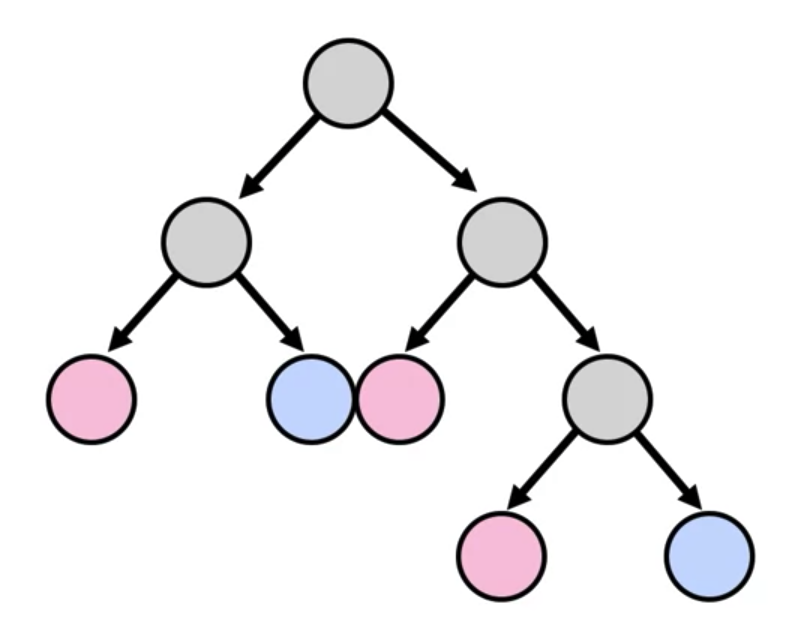
\includegraphics[width=1\textwidth]{./figures/dectree.png}
\caption{Decision tree layout}
\label{fig1}
\end{figure}

Decision Trees are used for both regression and classification problems. The goal is to create a model that predicts the value of a target variable by learning simple decision rules inferred from the data features. They start with the root of the tree and follow splits based on variable outcomes until a leaf node is reached and the result is given. Figure 6.2 details a visual representation of the decision tree layout. 

\subsection{Bootstrapping}

Bootstrapping is the process of randomly sampling subsets of a dataset over a given number of iterations and a given number of variables. These results are then averaged together to obtain a more accurate result. 

\subsection{Random Forest Regression}

\begin{figure}[h]
\centering
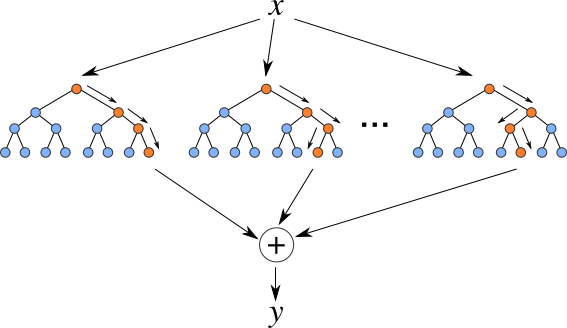
\includegraphics[width=1\textwidth, height=12cm]{./figures/rf.png}
\caption{Simple RF}
\label{fig1}
\end{figure}

The bootstrapping Random Forest algorithm \cite{B} combines ensemble learning methods with the decision tree framework to create multiple randomly drawn decision trees from the data, averaging the results to output a new result that often leads to strong predictions/classifications. Figure 6.2 documents a visual representation of random forest wherein \textbf{X} is the feature vector and \textbf{y} is the target vector. 

\section{MULTI LAYER PERCEPTRON}

The Multi Layer Perceptron bases its fundamental design to the interlinking of several neurons (like structures) representing a Neural Network (NN) architecture. Given $i = 0,1,..,n$ where n in the number of inputs, the quantities $w_{i}$ are the weights of the neuron. The inputs $x_{i}$ correspond to features or variables and the output y to their prediction/estimation. Figure 6.4 shows the simplified representation of the above steps.  

\begin{figure}[h]
\centering
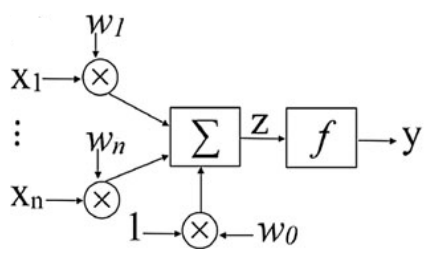
\includegraphics[]{./figures/perceptron.png}
\caption{Perceptron model}
\label{fig1}
\end{figure}

The weighting step involves the multiplication of each input feature value by its weight ${xiwi}$ and in the second step they are added together $(x_{0}w_{0} + x_{1}w_{1} + ... + x_{n}w_{n})$. The third is the transfer step where an activation function f (also called a transfer function) is applied to the sum producing an output y presented as:

\begin{equation}
    y = f(z)\;and\;z = \sum_{i=0}^{n} w_{i}x_{i}
\end{equation}

wherein $x_{0} = 0$, $w_{0}$ is the bias and y is the output. The activation function can be of the form of Unit step, Linear or Logistic operation. 

A perceptron can only learn linearly separable functions. For n dimensions, the function is a hyperplane with equation:

\begin{equation}
    \sum_{i=0}^{n} w_{i}x_{i} = 0
\end{equation}

The motive of learning is to optimize the weights by minimizing a cost function, which is usually a square error between the known vector and the estimated vector. Optimization techniques such as gradient descent algorithm can be used to determine the optimum weight vector. Ultimately, the algorithm converges to a solution reaching an operational configuration network. However, the perceptron and the single layer perceptron do not resolve the nonlinearly separable problem. 

\begin{figure}[h]
\centering
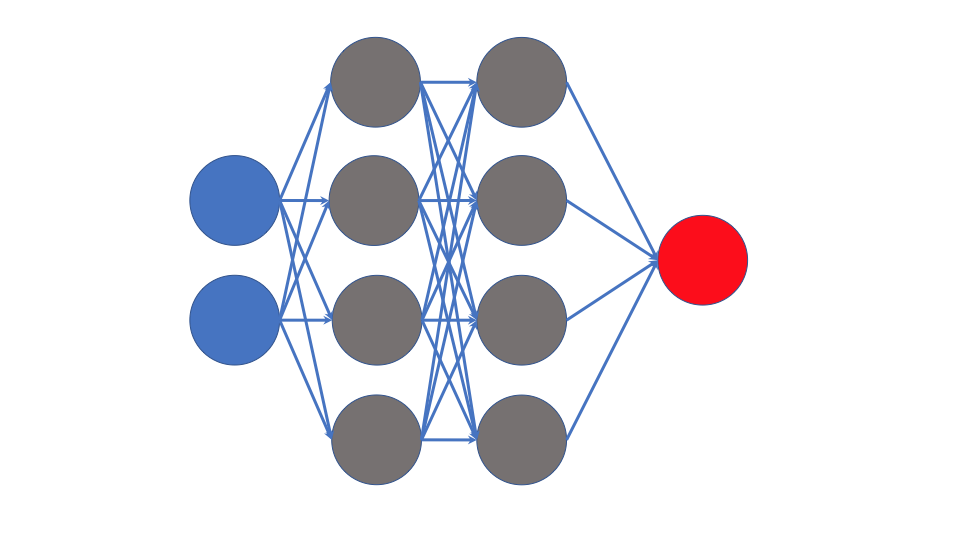
\includegraphics[width=1\textwidth]{./figures/mlp2.png}
\caption{MLP model}
\label{fig1}
\end{figure}

To solve this problem, Multi Layer Perceptron (MLP) architecture is created by aggregating layers of perceptrons wherein the output of one layer acts as the input of another layer. Multi Layer Perceptron \cite{C} is a feedforward neural network that consists of three layers, the input layer, the hidden layer and the output layer. Figure 6.5 presents an MLP with two inputs (blue), two hidden layers (grey) and one output (red). 

The input layer receives the input signal to be processed. The required task such as prediction and classification is performed by the output layer. An arbitrary number of hidden layers that are placed in between the input and output layer are the true computational engine of the MLP. Similar to a feed forward network in a MLP the data flows in the forward direction from input to output layer. The neurons in the MLP are trained with the back propagation learning algorithm, where the weights can be corrected by propagating the errors from layer to layer starting with the output layer and working backwards. MLPs are designed to approximate any continuous function and can solve problems which are not linearly separable.




